\documentclass[11pt, a4paper, oneside, openany]{book}

% Input and output encoding
\usepackage[utf8]{inputenc}
\usepackage[T1]{fontenc}

\usepackage[english]{babel}

\usepackage[dvipsnames]{xcolor}
\usepackage{lmodern}
\usepackage{enumitem}
\usepackage{todonotes}
\usepackage{setspace}
\usepackage{graphicx}
\usepackage{amssymb,amsmath}
\usepackage{mathtools}
\usepackage{float}
\usepackage[pass]{geometry}
\usepackage{ifdraft}


\definecolor{codebg}{rgb}{0.98, 0.98, 0.98} % light gray
\usepackage{minted}
\usemintedstyle{friendly}
\setminted{
    bgcolor=codebg,
    frame=single,
    fontsize=\small,
    xleftmargin=1em,
    framesep=0.5em
}



\usepackage[unicode=true,
    plainpages=false,
    pdfpagelabels,
    draft=false,
    colorlinks=true,
    hyperfootnotes=false,
    linkcolor={Sepia},
    citecolor={PineGreen},
    urlcolor={MidnightBlue},
]{hyperref}

\hypersetup{
    pdfauthor={Kirill Vorozhtsov},
    pdftitle={Musikk},
    pdfsubject={Bachelor's Thesis}
}

\usepackage[
    backend=biber,
    style=numeric,
    sorting=none,
    maxnames=100
]{biblatex}
\addbibresource{bibliography.bib}
\setlength{\tabcolsep}{6pt}

\usepackage{nameref}
\usepackage{adjustbox}
\usepackage{url}
% % % % % % % % % % % % % % % % % % % % % % % % % % % % % % % % % % % % % % % %

\begin{document}
    \frontmatter
    \pagestyle{empty}

\begin{center}
{\Large \textsc{Masarykova univerzita}}

{\large \textsc{fakulta informatiky}}
    \vskip4em
    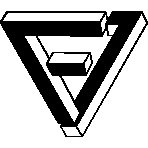
\includegraphics[width=4cm, height=4cm, draft=false] {logo_fi}
    \vskip4em
        {\begin{spacing}{1}
             \Huge \textbf{Musikk. A music streaming platform with social features.} % XXX: Title
    \end{spacing}}
    \vskip2em
        {\Large \textsc{Bachelor's Thesis}} % XXX: Type
    \vskip2em
        {\LARGE \textbf{Kirill Vorozhtsov}} % XXX: Author
    \vfill
    {\hfill\large Brno, 2025} % XXX: Year
\end{center}

\cleardoublepage
\restoregeometry

    \section*{Prohlášení} Prohlašuji, že tato práce je mým původním autorským dílem,
které jsem vypracoval samostatně. Všechny zdroje, prameny a literaturu, které
jsem při vypracování používal nebo z~nich čerpal, v~práci řádně cituji
s~uvedením úplného odkazu na příslušný zdroj.

\vfill\noindent
\textbf{Vedoucí práce:} Tvá babka   % XXX
\cleardoublepage

\section*{Poděkování} % XXX
\cleardoublepage

\section*{Shrnutí} % XXX

\subsection*{Klíčová slova} % XXX


    \setcounter{tocdepth}{2}
    \tableofcontents
    \pagestyle{plain}

    \mainmatter
    \chapter{Introduction}\label{chap:intro}


In recent years, with rapid development of the Internet,
music has become an even more integral part of everyday life.\cite{music_role_life}
It has never been easier to experience and share music — we have come
a long way from sharing vinyl records to simply sending a link to a streaming platform of choice.
Consequently, music has integrated even deeper into social interactions between people,
helping them bond and share strong emotional experiences.\cite{music_role_life}
\\
One of the direct impacts of this trend is the fast emergence of numerous music-related platforms.
While some focus on traditional music journalism or statistics, others offer unlimited access to audio content.
Naturally, people have started to discover and engage with music that resonates with them more frequently.\cite{music_role_life}
\\
Despite this, it is surprising that features which facilitate social interactions are not widely implemented in the
existing platforms, as will be shown in \nameref{chap:platforms}
\\
The goal of this thesis is to design a music-centric platform that embraces
collaboration and social interaction around music.
\\
This work is divided into the following \textbf{six} chapters:

\begin{enumerate}
    \item \textbf{\nameref{chap:survey}}
    Presents the outcomes of a survey illustrating how people consume music,
    how prevalent it is in social interactions, and why this thesis is relevant.

    \item \textbf{\nameref{chap:platforms}}
    Compares existing streaming solutions, music-related services
    and explores relevant non-musical platforms.

    \item \textbf{\nameref{chap:specs}}
    Outlines the functional and non-functional criteria for the application.

    \item \textbf{\nameref{ch:planning}}
    Describes the choices of technologies that are used by the application.

    \item \textbf{\nameref{chap:implementation}}
    Explains the development process and implementation details.

    \item \textbf{\nameref{chap:conclusion}}
    Summarizes the results and discusses possible improvements.
\end{enumerate}
    \chapter{Music Consumption Survey}\label{chap:survey}


\section{Background and objectives}
In order to better rationalize the topic of the thesis and show that a music streaming platform
is relevant as a service, a brief survey was conducted. It examines the
individual content‐consumption preferences, listening and discovery habits, platform usage patterns, and
social behaviours.


\section{Methods}
The platform chosen for the questionnaire was `Google Forms`\cite{googleforms}, as it provides a simple interface for
survey creation, allows for easy sharing of the form, and supports exporting the results to a spreadsheet.\\

The questionnaire itself consists of 15 questions.
Most of them are multi-choice and closed-ended with some having a possibility for a custom answer.\\

As for the respondents - 119 people had participated, with most being from Russian-speaking countries;
the majority was in the 18 to 30 age group, with the exact distribution shown in *fig.*

\subsection{Engagement}
Firstly, it was necessary to determine the actual frequency of engagement with audio content -- if the numbers were low,
it would indicate that a dedicated platform with advanced features might not be relevant for most users.
However, over 50\% of respondents reported listening to more than 500 songs per month *fig.*,
and nearly 80\% stated that they listen to music daily *fig.*.
This clearly shows that music is essential to many people, and the following logical step would be to discover
how the audio content is mostly accessed. \\

\subsection{Listening Methods}
As can be clearly seen in *fig* the percentage of streaming platforms usage across all ages is nearing 100\% with
slightly higher numbers in lower age groups. Although, downloaded files and physical media have their presence, especially for
people aged 30-60, it is usually only an auxiliary option next to the streaming solutions.
\\
Regarding the platforms themselves - Spotify has taken the first place in terms of popularity, proving the
global statistics\cite{spotifypopularity}. However, Yandex Music being in the second place deserves an explanation.
As mentioned previously, most of the respondents are from Russian-speaking countries, Russia specifically.
With a lot of western companies leaving its market in 2022, music streaming services included, most of the users has
moved to locally available services - Yandex Music, VK Music, Zvuk, and others.
Another notable point is the absence of other popular region-specific platforms, such as Amazon Music for the US market,
QQ music for the Chinese market or JioSaavn for the Indian one,
as all of the respondents were based in the european part of the world.
The full statistics are shown in *fig*.\\
Being established that streaming services are indeed widely-used and are in demand, the next important step would be
to analyze the regularity of music-centered social interactions.

\subsection{Social Interactions}
The results of Question 10 indicate that nearly all respondents (99.2\%) reported listening to music with
others, primarily in offline settings such as gatherings or car rides.
Online co-listening methods, while less common, were also mentioned by a quarter of respondents,
showing that digital solutions for shared listening are used, though not as prevalently as in-person scenarios.
\\
Question 11 investigates how often these interactions occur —
the results show that a significant portion of respondents engage in shared listening regularly.
Around 60\% reported doing so at least a few times per month,
with a smaller group indicating almost daily interactions.
This reinforces the idea that music consumption is a common social activity.
\\
The next question is phrased as following - "How often do you/your friends share/discuss music?".
While the previous question focused on real-time in-person collective listening,
this one highlights more intentional and in-depth musical interactions — such as sharing songs,
recommending music, or discussing it. Music in that case is not just the background but the main subject of engagement.
The same trend as before can be observed in the responses: a majority of participants reported engaging in these exchanges regularly.
Over 70\% indicated that they share music at least several times a month, with many doing so weekly or more often.
This further emphasizes the active social role of music.
\\
Question 13 — “How does that happen?” — provides an insight into the specific means of sharing.
Many respondents stated that they typically send links from streaming platforms through external messaging apps.
While this shows a clear demand for sharing music, it also reveals a gap: these interactions are fragmented across platforms.
Hence, enabling such exchanges directly within the streaming app could offer a smoother, more uniform experience.
\\
Responses to the question \textit{“Would you say that you know a lot of people with similar music taste?”} were mixed,
with a near-even split between those who do and do not.
This suggests that while some users already have a social circle with similar music taste, many do not.
Interestingly, when asked
\textit{“Would you like to connect with others who share your musical taste, or influence those around you to explore and appreciate the music you enjoy?”},
the majority answered positively.
This indicates a clear interest in expanding musical connections and supports the idea that social discovery
features could be useful within a streaming platform.
This is further supported by the responses to Question 15, where over 60\% of participants stated they would use
additional social features, if available on current streaming platforms.


\section{Results}
Overall, the results show that music is a vital part of many peoples' lives
and that streaming services are the main way people listen to it.
Music consumption is frequent, social, and often includes sharing and discovering new tracks.
Yet, current platforms only partly support these interactions.
Therefore, the idea of a music streaming service with integrated social features could be relevant,
addressing real user needs.


\begin{table}[ht]
    \label{tab:where_listen}
\end{table}
    \chapter{Existing Platforms}
In order to better understand what instruments people use when interacting with music,
it’s useful to examine existing solutions.


% TODO: add pictures for examples without links?


\section{Streaming Services}
% TODO: ref to survey table
As it can be seen from the table~\ref{tab:where_listen} and further confirmed by
the recent study of the International Federation of the Phonographic Industry\cite{music_stats_2024},
nowadays, the most prevalent way of music consumption
and discovery is the streaming services. There are many platforms available,
but only those that are both popular and feature unique elements will be considered.
The descriptions, rather than offering general information, will focus on the social aspects of each platform.

\begin{itemize}
    \item \textbf{Spotify} \\
    One of the most prominent social features on Spotify is the 'Spotify Jam'\cite{spotify_jam}.
    It lets people create a collective song queue which is then synchronized among all connected users.
    Moreover, volume, the order of songs and other aspects of the playback can be controlled individually.
    Another notable tool is the 'Blend' playlists\cite{spotify_recs}. These are playlists created automatically
    between two people, which contain songs matching audio preferences of both users.
    Lastly, 'Friend Activity'\cite{spotify_friend_activ}, which shows what the people you follow are currently listening to,
    and 'Listening Parties' that are live chats with a limited capacity,
    which can be joined for a short time when new music is being released\cite{spotify_party_1,spotify_party_2}.

    \item \textbf{VK Music} \\
    As was mentioned previously, this a music service integrated into the VK social network.
    Consequently, it is possible to send songs and playlists via private messages and add audio materials to
    posts in groups. VK Music also supports algorithmic playlists based on the groups that a user follows.
    It analyzes audio files posted in the specific groups and puts similar songs in those playlists.

    \item \textbf{SoundCloud} \\
    SoundCloud is one of the few platforms which lets its users leave comments
    and reactions on songs and playlists\cite{sc_comments,sc_reactions}.
    In addition, each user has a feed, consisting of his personal uploads and
    reposts of other's content\cite{sc_reposts}, which is visible when visiting his profile.

    \item \textbf{Bandcamp} \\
    Every Bandcamp user has a profile with 4 tabs - 'collection', 'wishlist', 'followers' and 'following'.
    By far the most interesting feature is under the `following` tab - users can subscribe to available genres and then
    specify the ones that they want to showcase to others viewing their profile.
    The ‘wishlist’ tab is also noteworthy,
    as Bandcamp’s model blends streaming with the traditional purchases of individual releases, and
    in this tab the user is able to show what he is looking forward to listening in the future.
\end{itemize}


\section{Forums, Blogs and other Music Media}
A lot of different resources are gathered under these umbrella terms - from professional music review websites to
amateur, personal pages.

\begin{itemize}
    \item \textbf{Rate Your Music} \\
    'Rate Your Music is one of the largest music databases online. It is an incredible tool that
    can help you find and learn about new music to listen to.'\cite{ryt}.\\
    This website is one of the biggest platforms with user-created content.
    Every member is able to write reviews and set ratings for music releases,
    contribute to the extensive 'wiki' consisting of genres, thematic lists and charts,
    and connect to other members of the forum. However, the content is still moderated,
    ensuring that only properly formatted reviews that do not violate guidelines can appear on the website.

    \item \textbf{2step.ru} \\
    One of the better representatives of 'old school' forums that is active to this day.
    This is a country-specific resource, and a consequence of that,
    on top of providing the regular music and forum components, there are elements which are usually missing
    from bigger portals. For example, a section about upcoming parties,
    a page dedicated to local and upcoming DJs, and an ongoing list of recorded radio shows.\cite{2step}

    \item \textbf{The Wire} \\
    The Wire is a long-running magazine with a strong online presence,
    known for its focus on experimental and underground music.
    Apart from conventional articles, reviews, and interviews it hosts podcasts, creates music compilations and curates
    video/photo collections.\cite{thewire}
\end{itemize}


\section{Other Platforms}
Another memorable outcome of the survey is the high percentage of music discovery on non-music specific platforms.
Instagram, YouTube, TikTok and other services that are able to host user-created content can have a major effect on
the listening habits. In recent years, music has been more deeply integrated into these platforms.
For instance, Instagram introduced a dedicated audio tool to seamlessly embed sounds and songs into ‘Reels’\cite{inst_audio},
while YouTube automatically detects songs used in videos and adds them to the video description.


\section*{Summary}
As it can be clearly seen, there are numerous instruments available across the Internet.
However, services offering audio content often lack many commonly used features,
forcing users to use multiple platforms in order to meet their needs. This project aims to bridge that gap,
particularly by enhancing the potential for social interaction among users.



    \chapter{Specification}\label{chap:specification}

In this chapter the general outline of the application is specified via functional and non-functional requirements.
The individual requirements are constructed based on the 'MoSCoW' criteria\cite{moscow}.


\section{Important Terms}

Below is the list of important terms that will be appearing throughout the requirements section.

\begin{itemize}
    \item \textbf{Anonymous User} – A User which is not yet registered in the system or has not logged in.
    \item \textbf{Artist} - a User with additional privileges.
    \item \textbf{User Profile} – An object which encompasses all the information related to a specific User.
    \item \textbf{Song} – An object representing an individual audio object.
    \item \textbf{Song Collection} – Represents a container that holds multiple Songs.
    \item \textbf{Playback} – A process during which the user is receiving audio information.
    \item \textbf{Playback Item} – A Song or a Song Collection.
    \item \textbf{Playback Queue} – A list of Playback Items.
    \item \textbf{Playback Device} – A device on which the app can be used.
    \item \textbf{Comment} – A small piece of text provided by the User input usually placed under a specific object to which it refers.
    \item \textbf{Reply Comment} – The same as Comment, but must be created in relation to another, 'parent' Comment.
    \item \textbf{Post} - A publication made by a User.
\end{itemize}
% TODO: add missing stuff

\clearpage


\section{Functional Requirements}

\begin{table}[h!]
    \centering
    \begin{tabular}{|p{12cm}|p{3cm}|}
        \hline
        \textbf{Requirement}                                                                                                                                            & \textbf{Priority} \\
        \hline
        The system shall support over-the-net audio Playback.                                                                                                           & Must Have         \\
        \hline
        The system shall provide a way to control the audio Playback. That includes shifting the Playback backward and forward, stopping the playback. & Must Have \\
        \hline
        The system shall provide a way to show Playback Items.                                                                                                          & Must Have         \\
        \hline
        The system shall support new Playback Item addition.                                                                                                            & Must Have         \\
        \hline
        The system shall provide a way to enqueue Playback Items and the means to manipulate the Playback Queue. & Must Have \\
        \hline
        The system shall make possible to add new Playback Devices and switch between them. & Must Have \\
        \hline
        The system shall have individual User Profiles.                                                                                                                 & Must Have         \\
        \hline
        The system shall allow Anonymous Users to create a User Profile and log in to the system using email and password. & Must Have \\
        \hline
        The system shall allow Users to change their User Profile information.                                                                                          & Must Have         \\
        \hline
        The system shall differentiate presented content based on the User. That includes Songs and Song Collections, User Profile information and other related items. & Must Have \\
        \hline
        The system shall allow for Song and Song Collection creation. Only Artists shall be allowed to create Songs. & Must Have\\
        \hline
        The system shall provide a way for Users to add Comments under Song Collections                                                                                 & Must Have         \\
        \hline
        The system shall provide a Post system. Posts shall be able to be created by Users. & Must Have \\
        \hline
        The system shall provide a way for Users to create relations to other Users. Post-related content shall be able to be filtered on these User relations. & Must Have \\
        \hline
        The system shall have a way to filter and search Playback Items and Users.                                                                                      & Must Have         \\
        \hline
        The system shall make it possible to create Reply Comments for Comments.                                                                                        & Should Have       \\
        \hline
        The system shall provide a notification system. It shall include Reply Comments and other appropriate items.                                                                                              & Should Have       \\
        \hline
        The system shall make it possible to filter Playback Items based on the User relations. & Should Have \\
        \hline
        The system shall provide chat capabilities.                                                                                                                     & Could Have        \\
        \hline
    \end{tabular}
    \caption{Functional Requirements}
\end{table}


\clearpage


\section{Non-functional Requirements}

\begin{table}[h!]
    \centering
    \begin{tabular}{|p{12cm}|p{3cm}|}
        \hline
        \textbf{Requirement}                                                                                                                                                               & \textbf{Priority} \\
        \hline
        The system shall provide access to its contents only to authorized Users. The only exception shall be the 'Log In/Sign Up' page. & Must Have \\
        \hline
        The system shall store content securely; data representation shall be as efficient as possible. & Must Have \\
        \hline
        The system shall store and transport sensible user information only in safe manners. & Must Have \\
        \hline
        The system shall, in case of failure, remain rendered on the screen and show the appropriate non-technical message to the User. & Must Have \\
        \hline
        The system shall render new available information without refreshing the content page. That includes new Comments, Playback Items, updated Playback Queue and other related items. & Must Have \\
        \hline
        The system shall provide a responsive search method which would react to dynamic user input. & Should Have       \\
        \hline
        The system shall synchronize Playback across multiple devices.                                                                                                                     & Should Have       \\
        \hline
    \end{tabular}
    \caption{Non-functional Requirements}
\end{table}

    \chapter{Implementation Planning}
This section provides an insight into the technology choices used to implement the application.
In addition, UML diagrams are provided as a high-level overview of the system.

The created platform is built using the Model-View-Controller\cite{11} architectural pattern.
It is split into three major parts:
- Backend. Implements all of the data-related logic and processing.
- API. Is responsible for transferring the data to the frontend and receiving commands from it.
- Frontend. Presents the data to the User and accepts his commands.


\section{Backend}
Python was chosen as the main language for the Backend part of the application.
It has support for all the needed instruments, such as calling external processes,
file handling, and executing asynchronous code. Moreover, it has a flexible and straightforward
syntax allowing for rapid development.
As this project is mostly IO-driven and most of the processor-heavy operations are offloaded to external processes,
i.e. no thread programming is used, Python's performance limitations\cite{12} will not have such a drastic effect.

\subsection{Framework Comparison}

Currently there are 3 well-developed and widely-used WEB frameworks available for Python:

\begin{itemize}
    \item \textbf{FastAPI.} \\
    'FastAPI is a modern, fast (high-performance), web framework for building APIs
    with Python based on standard Python type hints.'~\cite{13}. \\
    This framework offers a lightweight approach to API declaration, without adding almost no overhead.
    It has the best integration with API documentation standards such as
    Open API and API representation tools, e.g. Swagger.

    However, it is relatively new and barebones; given the requirements and the fact that
    still not many extra packages are available -
    a lot of custom code would have to be written on top, which is a disadvantage for this project.

    \item \textbf{Flask.} \\
    Flask is a micro framework based on the WSGI interface.
    It is well suited for smaller apps and takes a lean approach when it comes to choosing the components
    that will be used with it - most of the additional functionality is written by the community
    and is distributed as external packages.

    One of the main problems with Flask is that it does not integrate well enough with the ASGI
    interface which is practically necessary for proper handling of Server-Client path of communication.
    Moreover, using external packages for every almost bit of additional functionality can potentially be a security risk.

    \item \textbf{Django.} \\
    Django is a 'batteries-included' framework, in a sense that almost everything -
    from access control and database management to API routing and admin interface,
    is a part of it. Moreover, it has an extensive ecosystem with support for e.g. REST-style API
    design via \texttt{django-rest-framework}, different methods of Authentication,
    even different transfer protocols, such as websockets and Server Sent Events are available
    via the \texttt{django-channels} package and others that build on top of it.

    Some of the notable drawback are its opinionated design choices and the size of the application,
    as this framework includes a lot of parts that possibly will not be used.
\end{itemize}

Out of those three frameworks Django is the most suitable for the task.
The application will heavily rely on the database,
frontend will be written in React, hence a JSON-based API will be implemented,
moreover Django has a proper support for ASGI-based servers.

\subsection{Audio Representation and Streaming}

\subsection{Database}

\subsection{Authorization}

\subsection{Server-Client Communication}


\section{Frontend}
    \usepackage{hyperref}


\chapter{Implementation}\label{ch:implementation}

This chapter presents the created platform; it is structured somewhat similarly to the previous one - firstly, the
audio processing, representation and transfer are discussed, then both the backend and frontend are introduced,
and lastly, the deployment process is shown.
In addition, UML diagrams are provided as an overview of the system.

High level overview can be seen in the following~\ref{fig:system_overview},
~\ref{fig:backend},~\ref{fig:frontend} diagrams.

\begin{figure}[htbp]
    \centering
    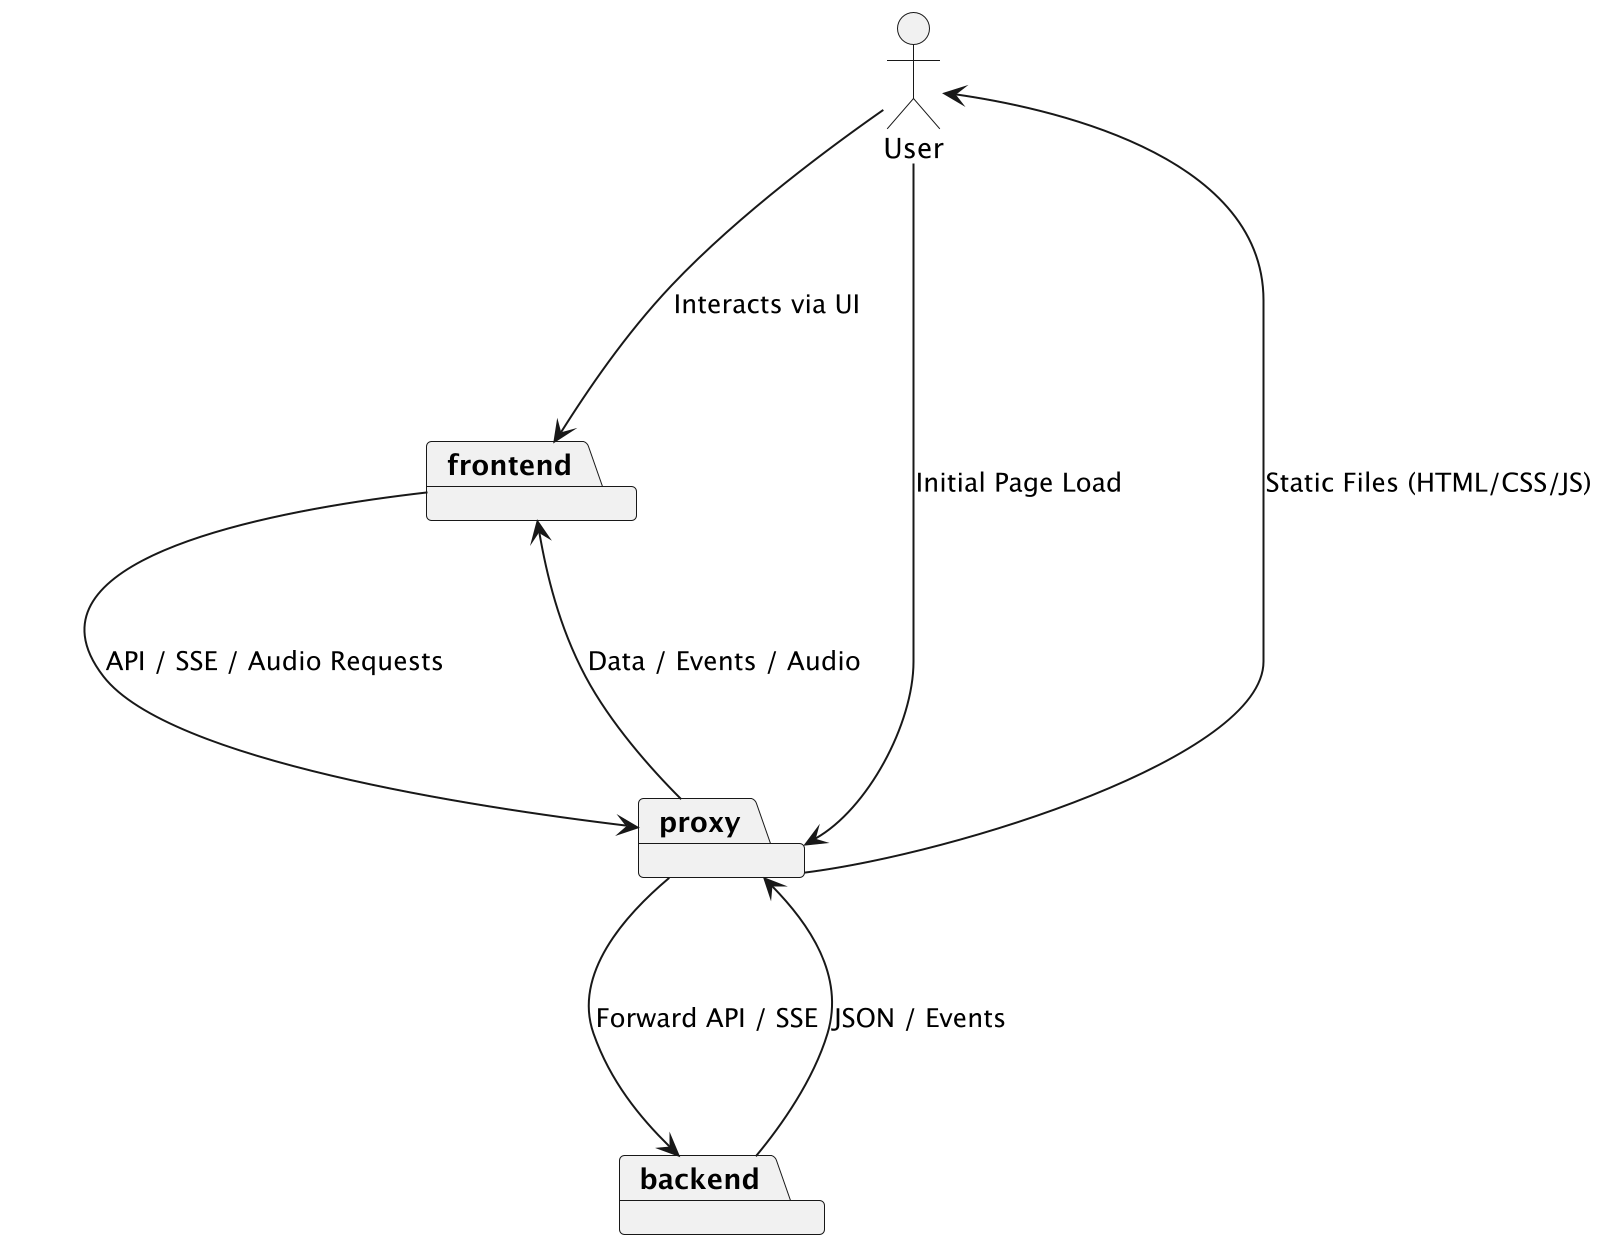
\includegraphics[width=1\textwidth, keepaspectratio]{diagrams/system.png}
    \caption{System Overview}
    \label{fig:system_overview}
\end{figure}

\begin{figure}[htbp]
    \centering
    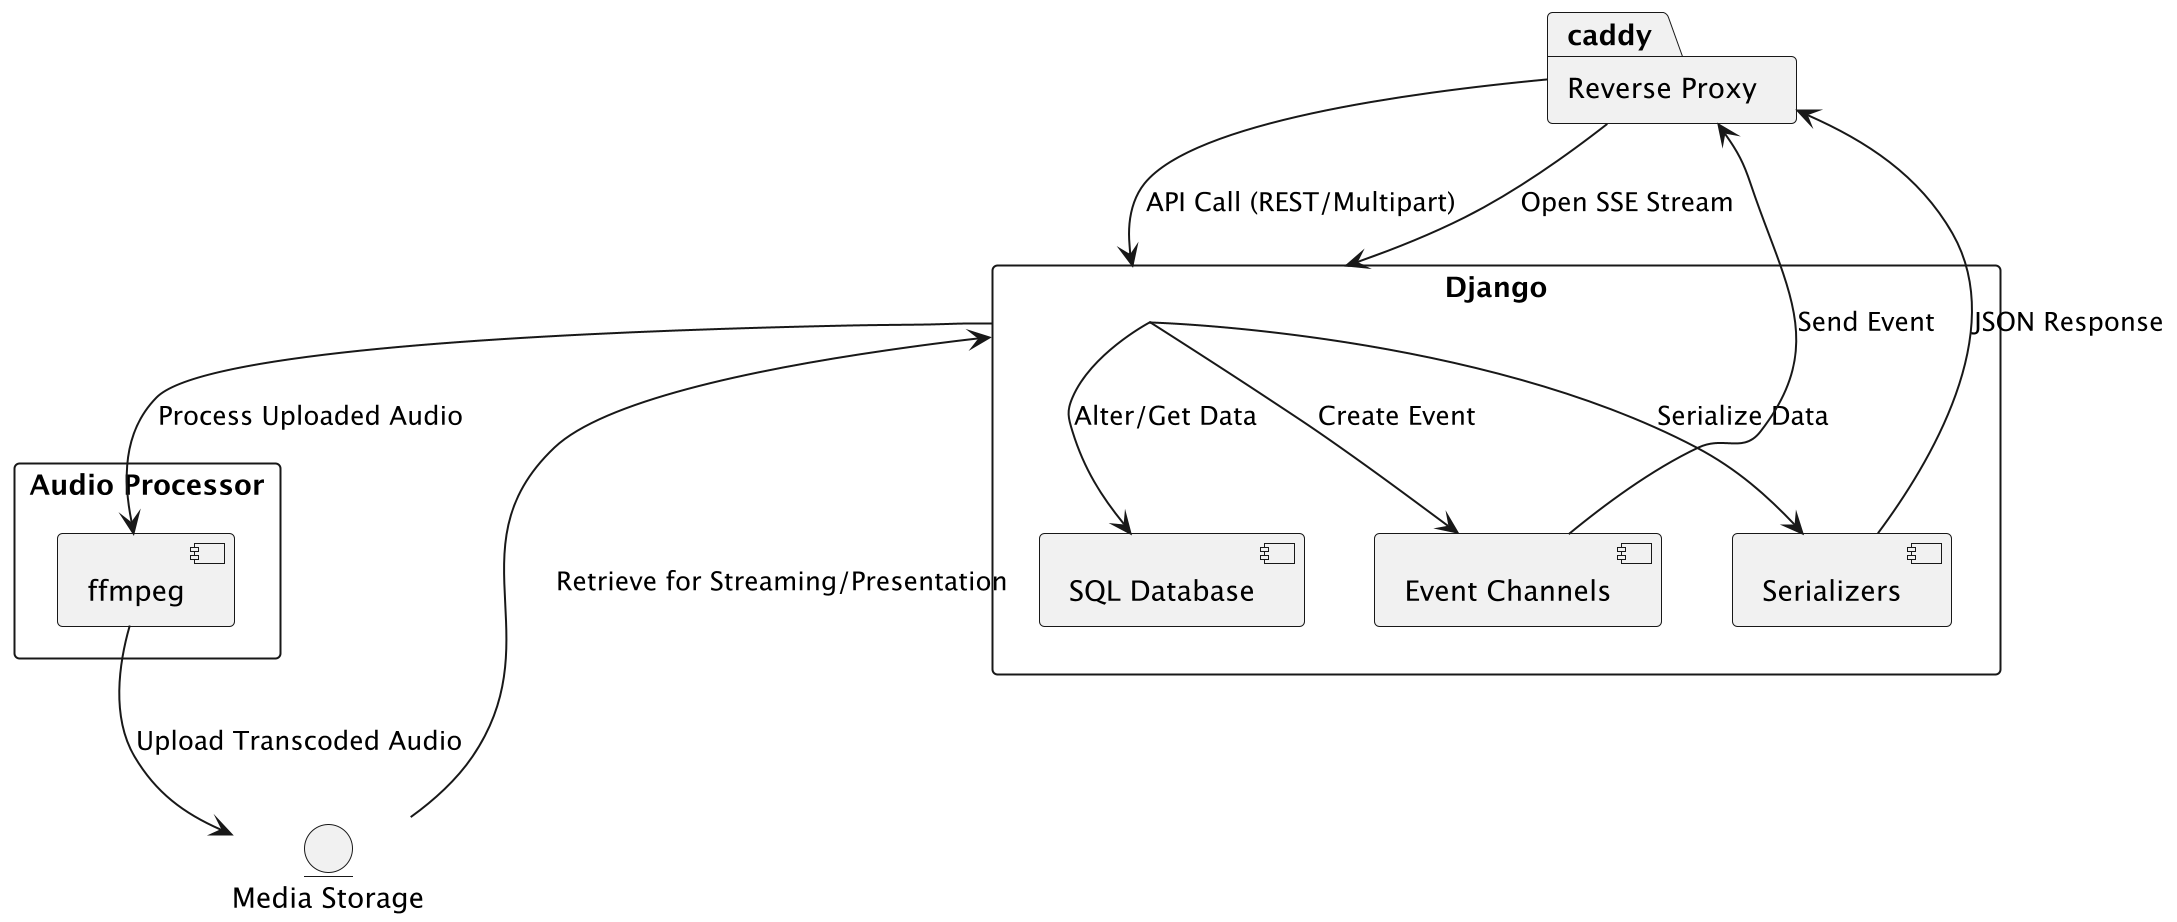
\includegraphics[width=1\textwidth, keepaspectratio]{diagrams/backend.png}
    \caption{Backend}
    \label{fig:backend}
\end{figure}

\begin{figure}[htbp]
    \centering
    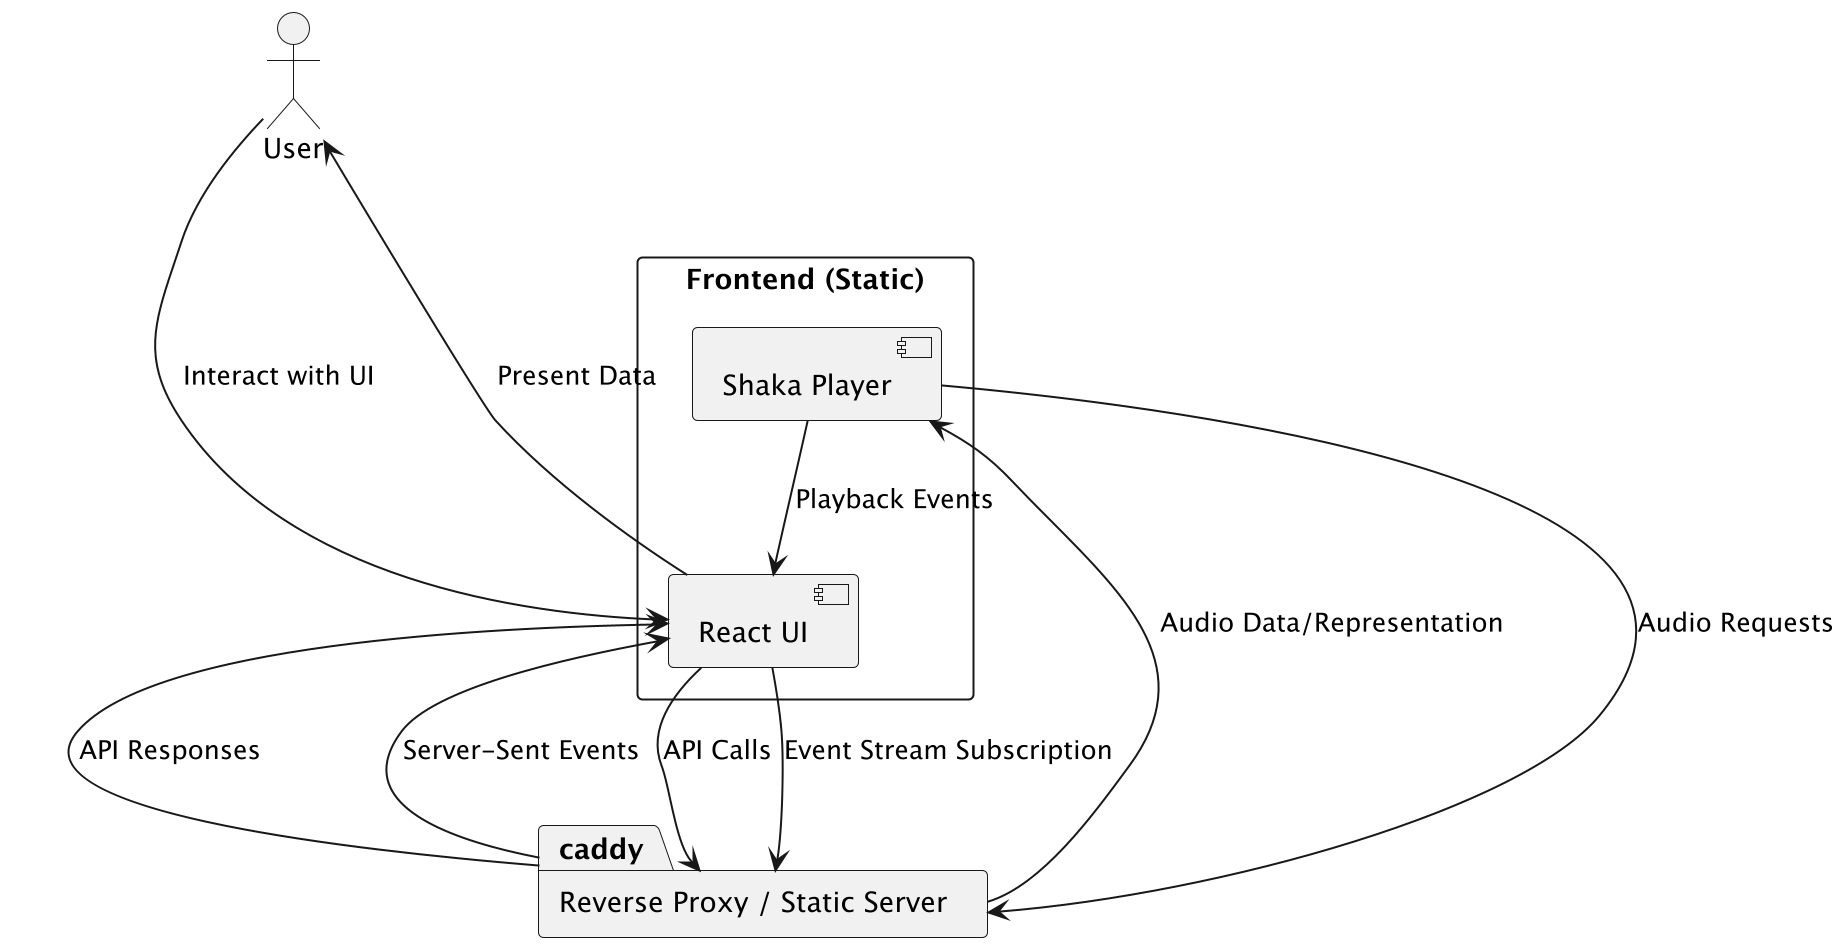
\includegraphics[width=1\textwidth, keepaspectratio]{diagrams/frontend.png}
    \caption{Frontend}
    \label{fig:frontend}
\end{figure}


\section{Audio Processing, Representation and Transfer}

\subsection{Streaming Protocols}
Two protocols were chosen for audio streaming - DASH\cite{dash} and HLS\cite{hls}.
Broadly speaking, they work by breaking the initial audio file into smaller chunks and present them via a manifest,
which is a listing with all available chunks separated by their timecodes. Then it is possible to use that manifest
to request individual chunks instead of fetching the whole file or its byte ranges. Moreover, it is possible to use
different coders and bitrates for the initial file, which would all be arranged together in the resulting manifest, giving
the possibility to choose which chunk will be served next - e.g. in the case of web audio players the next chunk can
be chosen based on multiple parameters, for example, network conditions.

At first, only DASH was considered, as it is codec and container agnostic,
is more efficient for lower bitrates, can stream lossless audio(HLS can only on Apple devices),
has multiple DRM implementations to choose from and many further advantages.
However, Safari does not support it well, and on iOS below 17.1 it does not work due to
Media Source Extensions~\cite{mse,msecaniuse} not being present.
Since Safari is the second most used browser~\cite{browserusage}, HLS is used as well.

After choosing the streaming protocols, it is needed to find the way of converting audio to formats that
they support. Audio representation is discussed first, with tools for the actual audio processing next.

\subsection{Representation}
Usually when audio is recorded, it is initially saved in lossless formats, which are big in size, due to
the absence of any compression. For instance, a the resulting WAV file for a 3-minute stereo audio
recorded with bit depth of 24 bits and a sample rate of 41khz is approximately 42 megabytes, which makes
it very impractical for over-the-net streaming.

Codecs are special programs which aim to reduce the size
while compromising audio quality as little as possible. Most often they take in multiple input parameters
which affect the resulting converted audio, among them is bitrate; the initial bitrate for the raw recorded audio
can be calculated as `Sample rate x Bit depth x Number of channels`.
However, codecs typically use bitrate as a primary input parameter instead of those individual components.
This is because bitrate directly controls the trade-off between audio quality and file size,
making it easier to manage both encoding and playback requirements.
It also abstracts away the internal implementation details, especially in lossy codecs like MP3, AAC, or Opus,
which use perceptual models and compression techniques that aren’t strictly tied to sample rate or bit depth.

The following configuration, based on the official documentation of the respective codec implementations, was selected:
\begin{itemize}[leftmargin=1.5cm]
    \item \textbf{Opus}: 96, 160, and 256 kbps for DASH
    \item \textbf{AAC}: 96, 160, and 320 kbps for HLS
    \item \textbf{AAC-HEv2}: 24 kbps for both HLS and DASH
\end{itemize}
According to performance measurements provided by the codec developers,
these bitrate values offer an optimal balance between audio quality and file size.
Multiple bitrates are included to support adaptive streaming,
allowing web players to dynamically select the most appropriate stream based on current conditions.

\subsection{Processing}
Audio processing is done via \texttt{ffmpeg}\cite{ffmpeg} which is a tool that support both the encoding of audio and the
manifest generation for both streaming protocols. It is written in C and supports multithreading ensuring high speed of
audio conversion.

FFMPEG provides multiple codec implementations, out of which \texttt{libfdk\_aac} and \texttt{libopus} were used.
Again, the choices made were backed by the documentation details~\cite{libfdkaac,libopus}.

In order to integrate it into the backend architecture a small wrapper was written, which can be found in the
\texttt{audio\_processing/ffmpeg\_wrapper.py} and \texttt{audio\_processing/converters.py} files; a class diagram is also
provided~\ref{fig:ffmpeg}.

\begin{figure}[htbp]
    \centering
    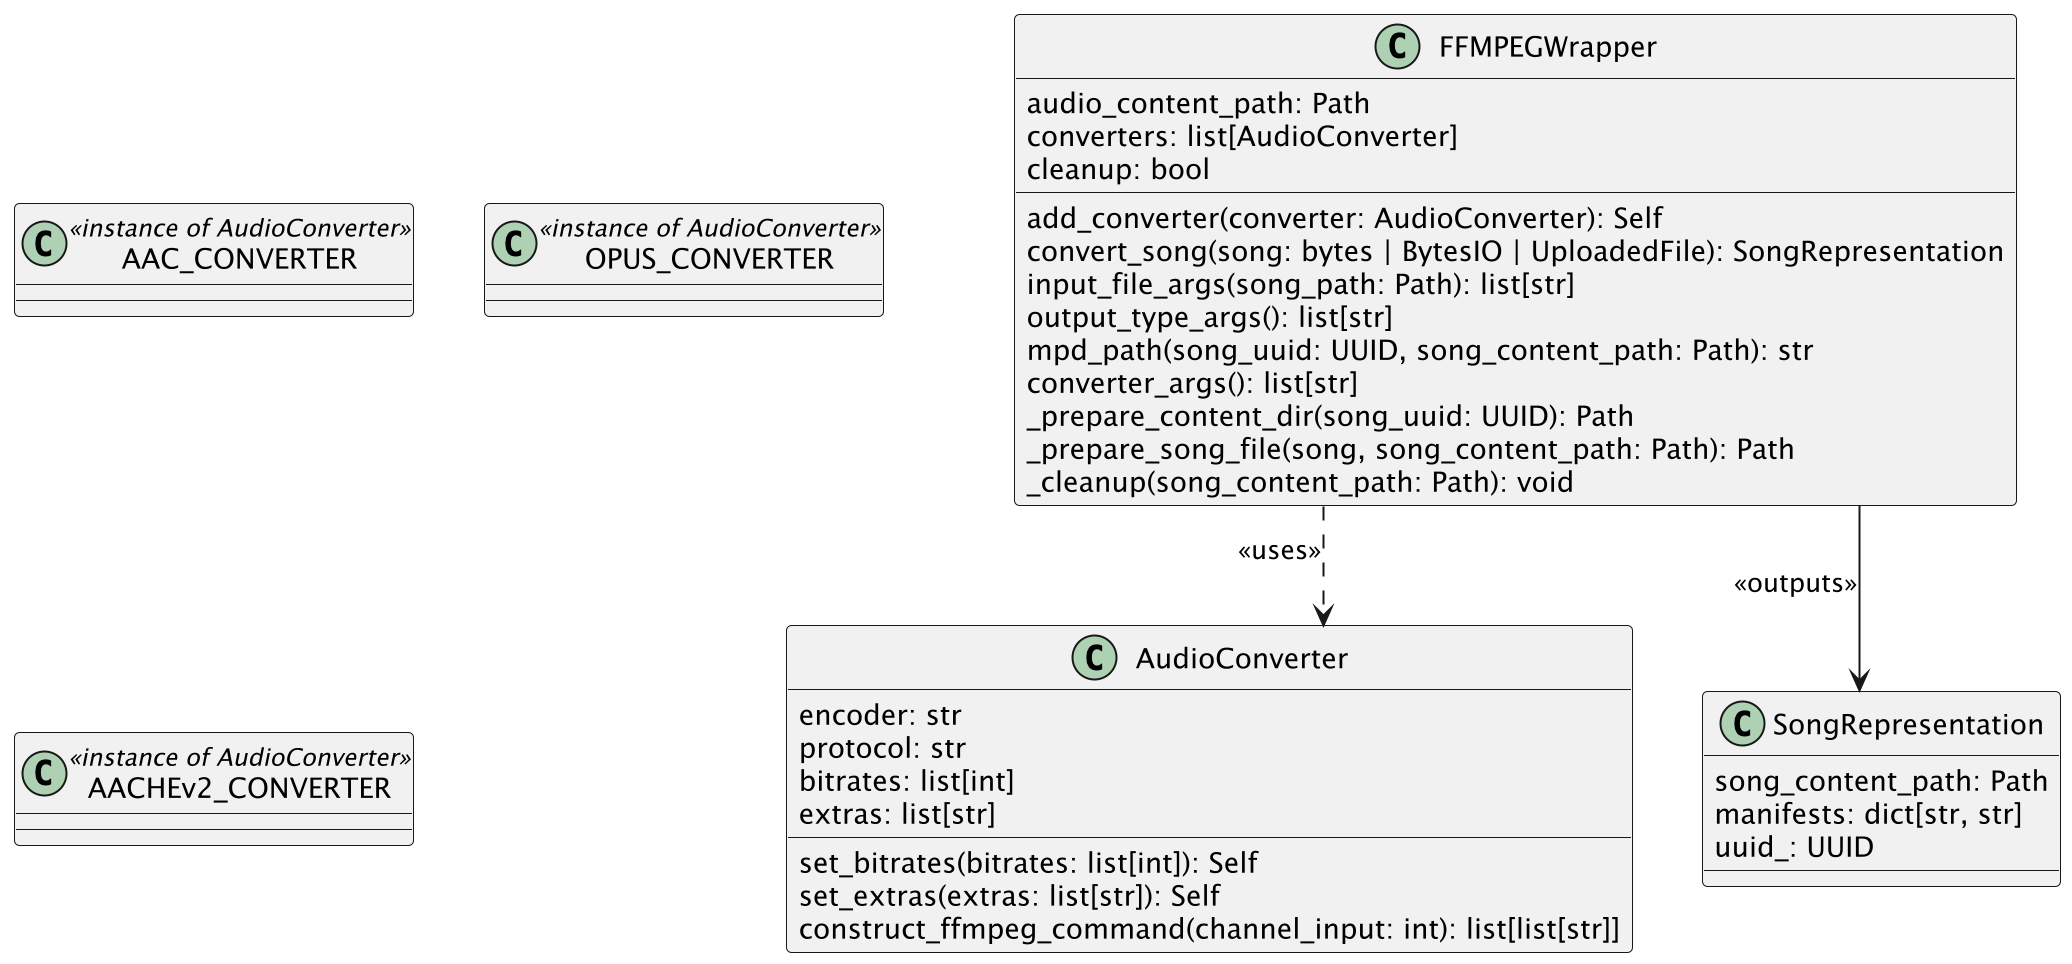
\includegraphics[width=1\textwidth, keepaspectratio]{diagrams/ffmpeg.png}
    \caption{FFMPEG Wrapper}
    \label{fig:ffmpeg}
\end{figure}

There are a couple of packages which already implement a wrapper around the library, however,
they are not used because the needed functionality is minimal and introducing a big
dependency is not necessary. In addition, the more popular and mature package \texttt{ffmpeg-python}\cite{ffmpegpython}
is not maintained anymore and e.g. OpenAI has dropped it as their dependency due to that reason\cite{ffmpegopenai}.

The resulting command for \texttt{ffmpeg} constructed by the wrapper(DASH only, for brevity) looks like this:

\begin{minted}{bash}
ffmpeg -i *input file path*
    -map 0:a -c:a:0 libfdk_aac -profile aac_he_v2 -b:a 24k
    -map 0:a -c:a:1 libopus -b:a 96k
    -map 0:a -c:a:2 libopus -b:a 160k
    -map 0:a -c:a:3 libopus -b:a 256k
    -f dash *output file path for manifest*
\end{minted}

\texttt{-map 0:a} tells \texttt{ffmpeg} to select the audio track(s) from the first input.

\texttt{-c:a:*} specifies the codec for each output audio stream.
The index (e.g., \texttt{:0}, \texttt{:1}, etc.) determines the order of the audio representations
in the output DASH manifest.

As the result, the individual manifests and corresponding chunks are created.
Later on they will be placed under a subdirectory
of Django's media directory, so they can later be served to the frontend audio player.

Having determined, how the audio is going to be processed and represented, backend implementation is
discussed in the further section.


\section{Backend}
The description is organized by individual Django \textit{apps}.
Each app section follows this structure:

\begin{enumerate}
    \item \textbf{Models} – Define the data schema using Django's ORM.
    \item \textbf{Serializers} – Convert Django models or native Python types into
    formats suitable for HTTP transmission (and vice versa).
    \item \textbf{API Endpoints} – Implemented as \textit{views}, these handle HTTP requests,
    apply the relevant business logic, and return appropriate responses.
\end{enumerate}

As a means to simplify the understanding of the underlying architecture, a full class diagram can be
seen first - it encompassed all attributes, methods and relationships of classes~\ref{fig:beclassdiagram}.

\begin{figure}[htbp]
    \centering
    \begin{adjustbox}{angle=90, width=1.4\textwidth, center}
        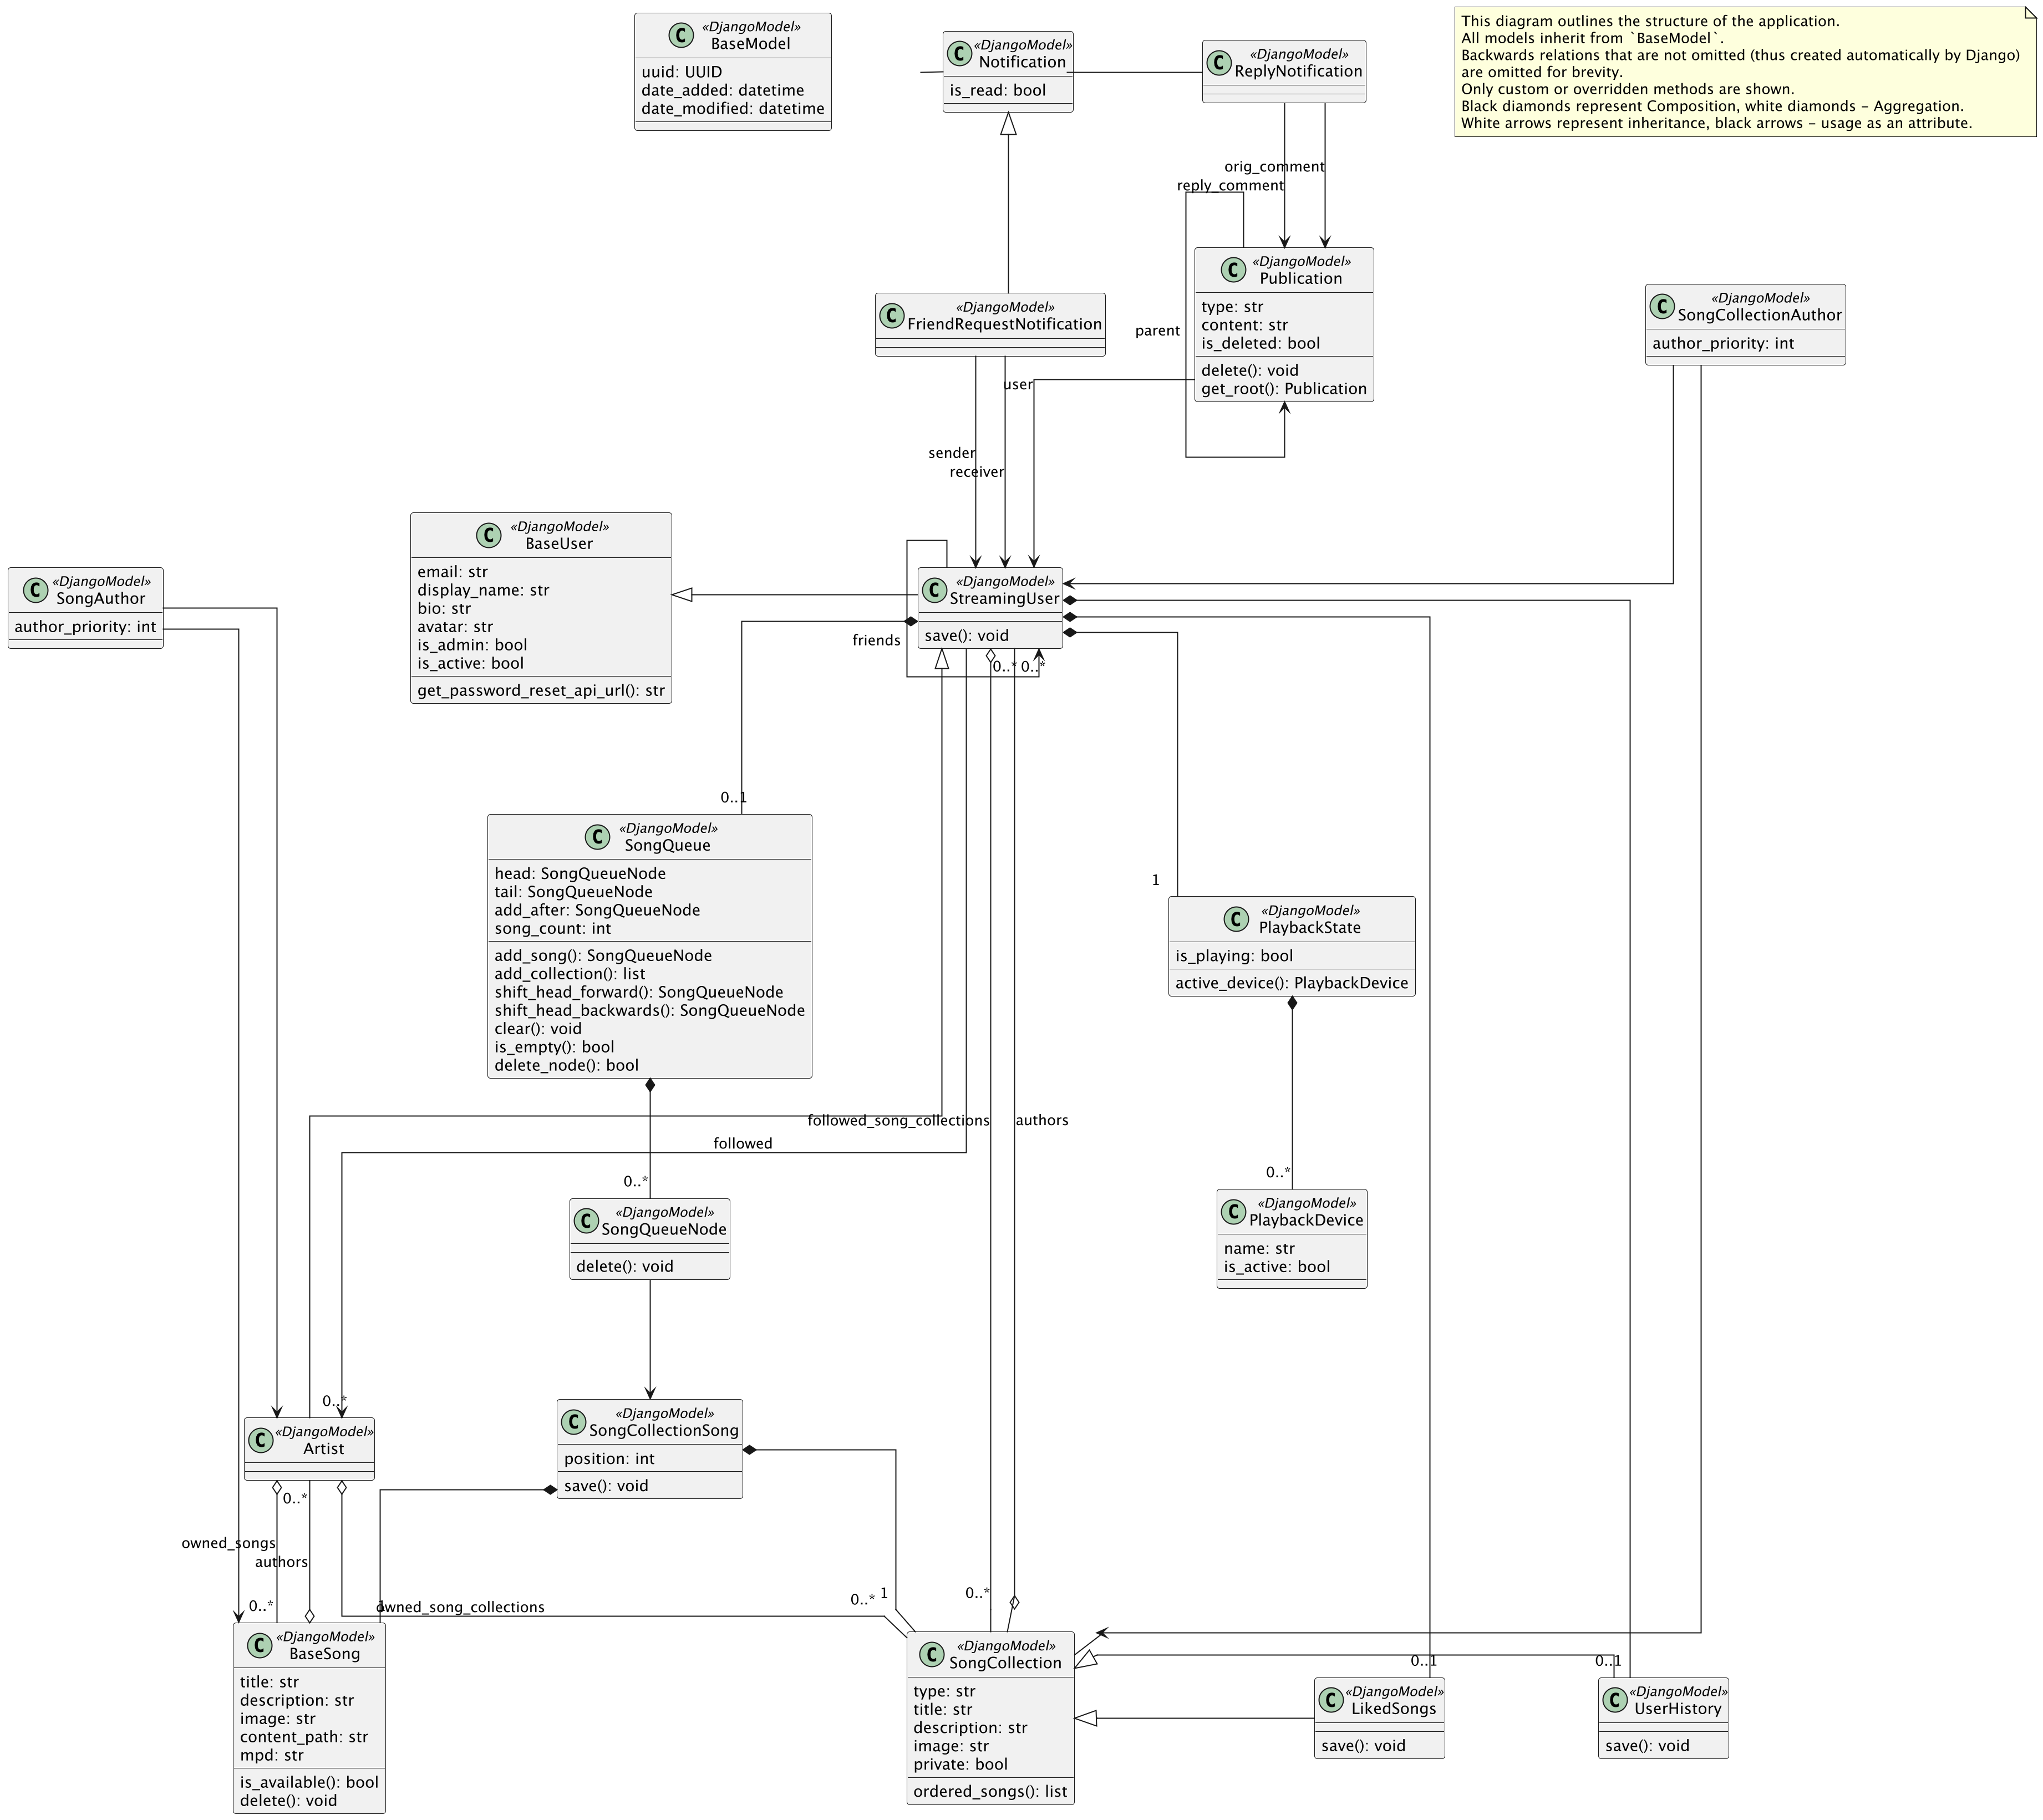
\includegraphics{diagrams/class.png}
    \end{adjustbox}
    \caption{Backend Class Diagram}
    \label{fig:beclassdiagram}
\end{figure}

\subsection{\textit{base}}
In this app the abstract \texttt{BaseModel} class is defined, all other models inherit from it.
It has three attributes - \texttt{uuid, date\_added, date\_modified}. While the latter two are self-explanatory,
\texttt{uuid} deserves an explanation. Since all of the data fetching in frontend will be happening via the REST API,
a unique resource identifier is needed.\\
The drawback of using an \texttt{ID} of the model record, which is added by default for all models by Django,
is the possibility of enumeration attacks~\ref{enumattack} and unauthorized scraping of the web page, since it is
much easier to get an existing ID and simply send requests to API endpoints with an incremented ID value.\\
A serializer for the model is defined here as well, it is also the base class for the serializers of other models.

\subsection{\textit{users}}
User classes and token logic are defined in this app.\\
There are three main User classes:
\begin{itemize}
    \item \texttt{BaseUser} - declares common fields for all other models, such as \texttt{email, display\_name} and others.
    \item \texttt{StreamingUser} - the main class representing an account with privileges to use the streaming platform.\\
    Additional attributes are declared for it, namely:
    \begin{itemize}
        \item Relations to other users: \texttt{friends}, which are other \texttt{StreamingUsers},\\
        friend requests of whom the user has accepted (or the other way around);\\
        \texttt{followed} - the \texttt{Artist}s to the updates of which the User has subscribed.
        \item User-specific Song Collections: \texttt{history} containing all listened Songs,\\
        \texttt{liked\_songs} containing favourited Songs,\\
        and \texttt{followed\_song\_collections} - the Collections which user has saved to their profile.
        \item \texttt{song\_queue} - a special structure containing already listened/to be listened to Songs of the User,\\
        it will be described later in the dedicated app.
    \end{itemize}
    \item \texttt{Artist}: a subclass of \texttt{StreamingUser} with additional capabilities, such as Song uploads.
\end{itemize}

JWTTokens are also customized in this app. The authentication process of individual HTTP requests is made by adding the
token to each request, then parsing and validating it. After validation the supplied User identifier is extracted and
is used to find the existing User record to which the request belongs. Thus, the \texttt{uuid} of the User is added to the token payload, and
the authorization logic, and it is customized to use UUID instead of ID for the user lookup.
The usage of UUID in the token payload will be described in more detail in the frontend section.

Basic serializers for all User models are declared,
allowing for the retrieval of information about specific Users or their creation and updates.

The following views are added as well:
\begin{itemize}
    \item \texttt{UserRetrieveUpdateView}
    \item \texttt{UserCreateView}
    \item \texttt{UserFriendsView}
    \item \texttt{UserFollowedView}
    \item \texttt{UserFriendsCreateDeleteView}
    \item \texttt{ArtistFollowersView}
    \item \texttt{UserEventViewSet}
\end{itemize}

The purpose of all views, except for the last one, could be deduced from their name.\\
UserEventViewSet is a special view used to implement the SSE connection, the details are provided in the next subsection.

\subsection{\textit{sse}}
As was mentioned in \nameref{ch:planning}, \texttt{django-eventstream} package is used for the Server Sent Events
configuration. Internally it works by creating special objects called \textit{channels} to which clients can subscribe
via an HTTP request. Then, when a new event for a specific channel is created,
e.g. via the \texttt{django-eventstream.send\_event()} method, all clients subscribed to that channel
will receive an HTTP response with the specified content.

`UserEventViewSet` listens for incoming SSE connection requests from Users and creates a personalized channel using User's UUID.

Events are mostly used throughout the system to signify to the frontend that some data is stale.
An example of this is the aforementioned `UserFriendsView`, the post request handler of which is defined like this:

\begin{minipage}{\textwidth}
    \begin{minted}{python}
    class UserFriendsCreateDeleteView(APIView):
    ...
    def post(self, request, *args, **kwargs):
        ...
        user.friends.add(sender)
        send_invalidate_event(
            EventChannels.user_events(user.uuid),
            ["user", "friends", str(user.uuid)]
        )
        ...
    \end{minted}
\end{minipage}
\\
\\
Here, the custom \texttt{invalidate\_event} signifies to the frontend that the \texttt{friends} list has changed and should
be refetched.

The \textit{invalidate} logic is used for models that are represented in the frontend,
specifically in view handlers which change data. That way the client always has fresh information.

Event re-delivery is also handled by the package, specifically with this parameter in Django settings:

\begin{flushleft}
    \begin{minted}{python}
    EVENTSTREAM_STORAGE_CLASS = \
        'django_eventstream.storage.DjangoModelStorage'
    \end{minted}
\end{flushleft}

This tells the package to store the events in the database, and in case of network failure or client disconnect they
are redelivered.

Since the SSE part has been explained, it is safe to move on to the main part of the application - the \textit{streaming} package.

\subsection{\textit{streaming}}


%
%\subsection{social}
%
%\subsection{recommendations}
%generic relations content type
%
%\subsection{notifications}
%
%\subsection{audio processing}
%
%\subsection{API}
%versioning, rest practices(and problems, e.g. action endpoints)
%using uuids
%
%
%\section{Frontend}
%
%\subsection{Libs used}
%tanstack query, shadcn, react router, form
%
%\subsection{Components}
%
%\subsection{Interacting with api}
%problems with on leave event
%
%\subsection{sse}
%
%\subsection{player}
%
%
%\section{Deployment}
    \chapter{Summary and Conclusion}
    \backmatter


    \chapter{Sources}
    \begingroup
    \raggedright
    \printbibliography[heading=none]
    \endgroup


\end{document}
